\chapter{传递函数}

上一章讲到由于拉普拉斯变换的特性使得用拉普拉斯形式可以将系统的时域的微分方程转化为多项式。
本章着重LT的工程应用——判断系统的稳定性和频率响应函数。

所谓稳定性,即系统对于输入结束后,其输出能否回归到0。
如果稳定性判断放在时域,则需要求解微分方程,得到系统输出的表达式,进而判断,但通过LT,可以放在s域判断,除此之外还能计算系统达到稳定后的输出。

频率响应函数和信号的FT本质上是一致的,都是频域的描述。
前者是对系统的描述,后者是对信号的描述。
通过频率响应函数,将系统和信号结合在一起,以在频域角度考察系统对信号的作用。

本章要点:
\begin{itemize}
    \item 传递函数。
    \item 系统的稳定性。
    \item 频率响应函数。
    \item 波特图。
\end{itemize}

\newpage
\section{传递函数的概念}

拉普拉斯变换的应用是描述系统,能将复杂的微分方程化为简单的加减乘除。
传递函数就是在复频域描述系统的微分方程。

本节要点:
\begin{itemize}
    \item 从微分方程和卷积的角度理解系统传递函数;
    \item 熟悉使用传递函数描述系统。
\end{itemize}

%============================================================
\subsection{从卷积到传递函数}

\begin{definition}[传递函数]
如果一个零状态LTI系统对于信号$x\left( t \right) $的输出可以表示为卷积:
\[
y\left( t \right) =x\left( t \right) \ast h\left( t \right)
\]
根据LT的卷积性质可以得到:
\[
Y\left( s \right) =X\left( s \right) \cdot H\left( s \right)
\]
\begin{itemize}
    \item $x\left( t \right) ,y\left( t \right) $:输入输出信号的时域表达式;
    \item $h\left( t \right) $:系统的冲激响应;
    \item $X\left( s \right) ,Y\left( s \right) $:输入输出信号的拉普拉斯变换;
    \item $H\left( s \right) $:{\bf 系统的传递函数}(transfer function),即系统对冲激响应的拉普拉斯变换$h\left( t \right) \leftrightarrow H\left( s \right) $。
\end{itemize}
\end{definition}

可见,只要是LTI系统,其冲激响应和传递函数是一一对应关系。
任何LTI系统都有且仅有一个独有的冲激响应,也必然有且仅有一个传递函数。
从数学角度看,LT和FT一样都是空间变换。

相比于傅里叶变换中的系统频域响应定理,这里不要求$h\left( t \right) $满足绝对可积的条件。
和FT一样,LT中也有冲激响应的变换结果$h\left( t \right) \leftrightarrow H\left( s \right) $,只是LT中称为传递函数,数学上两者都是对冲激信号的变换。
但FT的物理意义侧重于对信号本身的变换,故称为频率响应函数,而LT侧重于系统对信号的处理这一行为的变换,故称为传递函数。

%============================================================
\subsection{从微分方程到传递函数}

\begin{definition}[传递函数]
对于所有的有限维度LTI系统,我们必然可以用线性常系数微分方程描述,如下:
\[
y^{\left( n \right)}\left( t \right) +\sum_{i=0}^{n-1}{A_iy^{\left( i \right)}\left( t \right)}=\sum_{i=0}^m{B_ix^{\left( i \right)}\left( t \right)}
\]
若系统还满足:
\begin{itemize}
    \item 无初始能:$y\left( 0^- \right) =y'\left( 0^- \right) =\cdots =y^{\left( n-1 \right)}\left( 0^- \right) =0$;
    \item 0刻之前无输入信号:$x\left( 0^- \right) =x'\left( 0^- \right) =\cdots =x^{\left( m-1 \right)}\left( 0^- \right) =0$;
    \item 系统满足因果律。
\end{itemize}
则输出的拉普拉斯变换有:
\[
Y\left( s \right) =\frac{B_ms^m+\cdots +B_1s+B_0}{s^n+A_{n-1}s^{n-1}+\cdots +A_1s+A_0}\cdot X\left( s \right)
\]
我们称
\begin{align*}
H\left( s \right) &=\frac{B_ms^m+\cdots +B_1s+B_0}{s^n+A_{n-1}s^{n-1}+\cdots +A_1s+A_0} \\
&=\frac{B_m\left( s-z_1 \right) \left( s-z_2 \right) \cdots \left( s-z_m \right)}{\left( s-p_1 \right) \left( s-p_2 \right) \cdots \left( s-p_n \right)}
\end{align*}
为该{\bf 有限维度因果LTI系统在零状态下的传递函数}。
同时,$z_1,z_2,\cdots ,z_m$称为{\bf 系统的零点},$p_1,p_2,\cdots ,p_n$称为{\bf 系统的极点}。
\end{definition}

这样的系统的传递函数必然是一个有理式。
反之亦然,如果一个因果LTI系统的传递函数是有理式,则必然是有限维度。
其次,上述讨论也可看出,系统的微分方程的系数直接就是传递函数的系数。

如果输出是输入的积分,则可先两边求导,再取LT:
\begin{align*}
&y\left( t \right) =y\left( 0 \right) +\int_0^t{x\left( \tau \right) d\tau} \\
&\frac{d}{dt}y\left( t \right) =x\left( t \right) \leftrightarrow sY\left( s \right) -y\left( 0 \right) =X\left( s \right)
\end{align*}
如果系统零状态,则:
\[
Y\left( s \right) =\frac{1}{s}X\left( s \right)
\]

%============================================================
\subsection{零极点图}

将系统传递函数的零点和极点在复平面标记出来,得到的图称为{\bf 零极点图}(pole-zero diagram)。

~

\begin{example}
若传递函数如下,画出其零极点图。
\[
H\left( s \right) =\frac{s^2-2s+1}{s^3+3s^2+4s+2}
\]
\end{example}

首先用Numpy的roots()函数求出零点和极点。

\begin{python}
import numpy as np

B = np.roots([1,-2,1])
A = np.roots([1,3,4,2])

=====output=====
B = [1. 1.]
A = [-1.+1.j -1.-1.j -1.+0.j]
\end{python}

画出零极点图:
\begin{figure}[h]
\centering
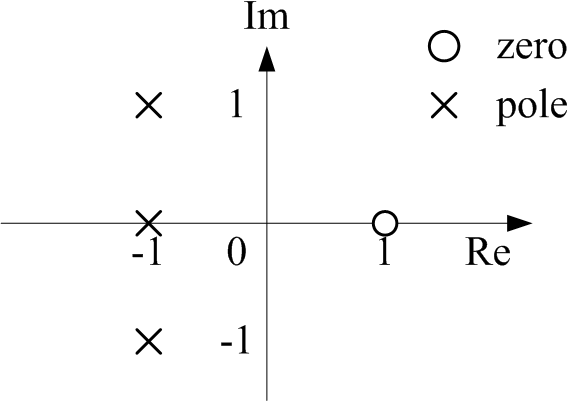
\includegraphics[height=3.5cm]{8.1.3-1.png}
\end{figure}

%============================================================
\subsection{系统框图}

并联系统(parallel interconnection)
\begin{figure}[h]
\centering
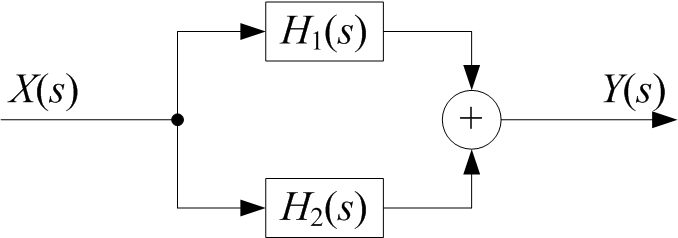
\includegraphics[height=2cm]{8.1.4-1.png}
\end{figure}
\[
H\left( s \right) =H_1\left( s \right) +H_2\left( s \right)
\]

串联系统(series interconnection),也称级联(cascade interconnection)
\begin{figure}[h]
\centering
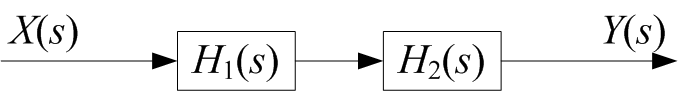
\includegraphics[height=0.8cm]{8.1.4-2.png}
\end{figure}
\[
H\left( s \right) =H_1\left( s \right) \cdot H_2\left( s \right)
\]

负反馈系统(negative feedback interconnection)
\begin{figure}[ht]
\centering
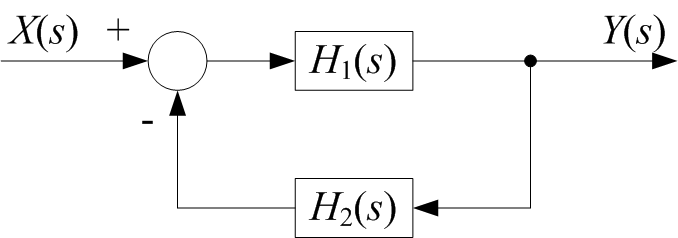
\includegraphics[height=2cm]{8.1.4-3.png}
\end{figure}
\[
H\left( s \right) =\frac{H_1\left( s \right)}{1+H_1\left( s \right) \cdot H_2\left( s \right)}
\]

%============================================================
\subsection{Python应用——scipy.signal中的传递函数类}

scipy.signal.lti()用零极点的方式生成传递函数类。
\begin{figure}[h]
\centering
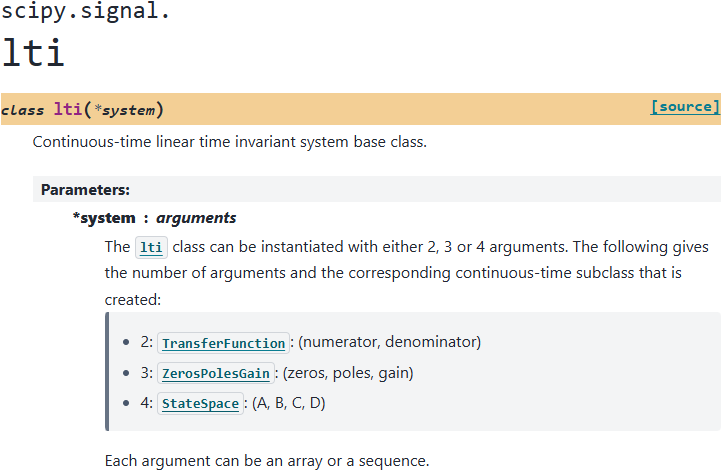
\includegraphics[width=8cm]{8.1.5-1.png}
\end{figure}

scipy.signal.TransferFunction()用多项式的方式生成传递函数类。
\begin{figure}[h]
\centering
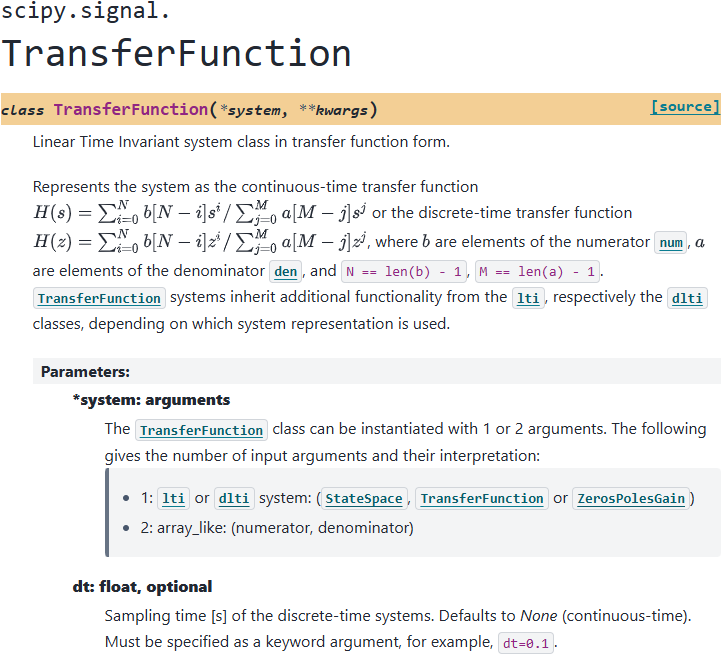
\includegraphics[width=8cm]{8.1.5-2.png}
\end{figure}

~

\begin{example}
\[
H\left( s \right) =\frac{5\left( s-1 \right) \left( s-2 \right)}{\left( s-3 \right) \left( s-4 \right)}
\]
\end{example}

\begin{python}
>>> scipy.signal.lti([1, 2], [3, 4], 5)
ZerosPolesGainContinuous(
array([1, 2]),
array([3, 4]),
5,
dt: None
)
\end{python}

~

\begin{example}
\[
H\left( s \right) =\frac{s^2+3s+4}{s^2+2s+1}
\]
\end{example}

\begin{python}
>>> num = [1,3,4]
>>> den = [1,2,1]
>>> scipy.signal.TransferFunction(num, den)
TransferFunctionContinuous(
array([1., 3., 4.]),
array([1., 2., 1.]),
dt: None
)
\end{python}

%============================================================
\subsection{电路中的传递函数}

\begin{tcolorbox}
很多情况下,我们不需要通过微分方程获得系统传递函数。
而是通过分析构成系统的组件的时域表达式,将其转换为s域表达式,然后根据组件之间的串并联及反馈的拓扑关系直接写出传递函数。
\end{tcolorbox}

以电路为例,首先将基本元器件(电阻、电容、电感)的电压电流关系式两端分别作LT,得到它们的s域表达式:
\[
\begin{array}{l}
	u\left( t \right) =Ri\left( t \right)\\
	\frac{du\left( t \right)}{dt}=\frac{1}{C}i\left( t \right)\\
	u\left( t \right) =L\frac{di\left( t \right)}{dt}\\
\end{array}\overset{\mathscr{L}}{\longleftrightarrow}\begin{array}{l}
	U\left( s \right) =RI\left( s \right)\\
	U\left( s \right) =\frac{1}{sC}I\left( s \right) +\frac{1}{s}u\left( 0 \right)\\
	U\left( s \right) =sLI\left( s \right) -Li\left( 0 \right)\\
\end{array}
\]
\begin{itemize}
    \item $u\left( t \right) ,i\left( t \right) $:元件两端电压,流经元件的电流;
    \item $U\left( s \right) ,I\left( s \right) $:$u\left( t \right) ,i\left( t \right) $的LT;
    \item $u\left( 0 \right) $:电容的初始电压;
    \item $i\left( 0 \right) $:电感的初始电流。
\end{itemize}
特别地,当电路系统无初始储能时(电容无储电,电感无磁能),它们的s域表达式为:
\[
\begin{array}{l}
	u\left( t \right) =Ri\left( t \right)\\
	\frac{du\left( t \right)}{dt}=\frac{1}{C}i\left( t \right)\\
	u\left( t \right) =L\frac{di\left( t \right)}{dt}\\
\end{array}\overset{\mathscr{L}}{\longleftrightarrow}\begin{array}{l}
	U\left( s \right) =RI\left( s \right)\\
	U\left( s \right) =\frac{1}{sC}I\left( s \right)\\
	U\left( s \right) =sLI\left( s \right)\\
\end{array}
\]
由于这三类元器件组成的系统为因果的LTI系统,符合传递函数的串并联定理,所以由电阻、电容、电感在s域可以视为“普通的”线性元件从而进行串并联。

也可以认为基尔霍夫定律在s域也是成立的。

~

\begin{example}
以RC电路例,假设电路零状态,$x\left( t \right) =1\mathrm{V},R=1\Omega ,C=1\mathrm{F}$,计算系统在0~10S这段时间内的输出。
\begin{figure}[h]
\centering
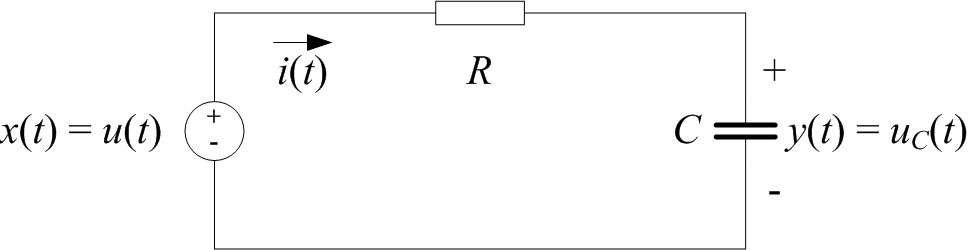
\includegraphics[height=2cm]{1.5.1-1.png}
\end{figure}
\end{example}

系统传递函数:
\[
H\left( s \right) =\frac{\frac{1}{sC}}{R+\frac{1}{sC}}=\frac{1}{sRC+1}=\frac{1}{s+1}
\]
输入$x\left( t \right) =1\mathrm{V}$视为单位阶跃信号,用Scipy库的signal模块的step()函数可以画出系统对单位阶跃信号的时域响应。

\begin{python}
H    = signal.lti([1],[1,1])
t, y = signal.step(H, T=np.arange(0,10,0.1))

ax.plot(t, y)
\end{python}

\begin{figure}[h]
\centering
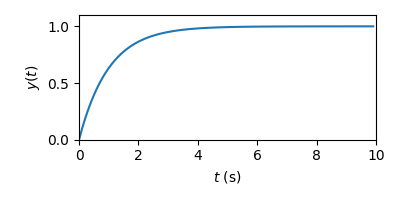
\includegraphics[height=3cm]{8.1.6-1.png}
\end{figure}

~

\begin{example}
如下电路,设输入为电压源电压,输出为流经电容$C_1$的电流,求系统的传递函数。
\begin{figure}[ht]
\centering
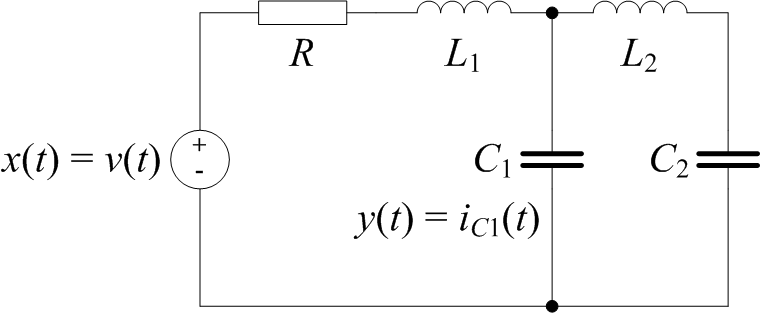
\includegraphics[height=2.5cm]{8.1.6-2.png}
\end{figure}
\end{example}

假设$C_1$的电压的LT为$U\left( s \right) $,有:
\begin{align*}
&\because Y\left( s \right) =\frac{V\left( s \right)}{1/sC_1}=\frac{\left( sL_2+1/sC_2 \right) \parallel 1/sC_1}{R+sL_1+\left( sL_2+1/sC_2 \right) \parallel 1/sC_1}X\left( s \right) \cdot sC_1 \\
&\therefore H\left( s \right) =\frac{\left( sL_2+\frac{1}{sC_2} \right) \parallel \frac{1}{sC_1}}{R+sL_1+\left( sL_2+\frac{1}{sC_2} \right) \parallel \frac{1}{sC_1}}\cdot sC_1
\end{align*}






\newpage
\section{系统的冲激响应及稳定性}

本节讨论传递函数的用途之一——稳定性判断。

本节要点:
\begin{itemize}
    \item 充分理解系统响应函数和传递函数本质上的一致性;
    \item 理解稳定的定义;
    \item 理解稳定性判据;
    \item 掌握使用稳定性判据判断系统稳定性。
\end{itemize}

%============================================================
\subsection{系统的冲激响应及稳定性要求}

假设LTI系统的传递函数$H\left( s \right) $,对于单位阶跃信号$\delta \left( t \right) $的响应:
\begin{align*}
&\because \delta \left( t \right) \leftrightarrow 1 \\
&\therefore Y\left( s \right) =H\left( s \right) \cdot 1=H\left( s \right) \\
&\therefore y\left( t \right) =h\left( t \right)
\end{align*}
可见,LTI系统对于冲激信号的响应即为传递函数的iLT,两者是等价的。

\begin{definition}[系统的稳定性]
当一个LTI系统对于冲激信号,当时间足够长后,输出为0,我们称{\bf 系统稳定}(stable),如果输出不为0但有界,称系{\bf 统临界稳定}(marginally stable),如果输出发散,称{\bf 系统不稳定}(unstable)。
\[
\underset{t\rightarrow +\infty}\lim y\left( t \right) =\begin{cases}
	0 &\mathrm{stable}\\
	C &\mathrm{marginal} \,\, \mathrm{stable}\\
	\infty &\mathrm{unstable}\\
\end{cases}
\]
由于零状态LTI系统的冲激响应为$h\left( t \right) $,所以系统输出的稳定性也可以表示为冲激响应函数的敛散性:
\[
\underset{t\rightarrow +\infty}\lim h\left( t \right) =\begin{cases}
	0 &\mathrm{stable}\\
	C &\mathrm{marginal} \,\, \mathrm{stable}\\
	\infty &\mathrm{unstable}\\
\end{cases}
\]
\end{definition}

通俗来讲,就是当输入结束后,输出能不能降到0。

%============================================================
\subsection{系统的稳定性判据}

\begin{theorem}[LTI系统的稳定性判据]
假设零状态LTI系统有传递函数:
\[
H\left( s \right) =B\frac{\left( s-z_1 \right) \left( s-z_2 \right) \cdots \left( s-z_m \right)}{\left( s-p_1 \right) \left( s-p_2 \right) \cdots \left( s-p_n \right)} \qquad m<n
\]
则$H\left( s \right) $的极点反应了系统冲激响应的形状,具体来说有:
\begin{itemize}
    \item 对于实数单极点$p$,冲激响应包含增益项$ce^{pt}$;
    \item 对于复数共轭极点$p,\bar{p}$,冲激响应包含振荡项$2\left| c \right|e^{\sigma t}\cos \left( \omega t+\angle c \right) $;
    \item 对于重复极点,冲激响应包含$t$次方的多项式。
\end{itemize}
当$H\left( s \right) $所有极点满足$\mathrm{Re}\left[ p_i \right] <0$时,即均出现在零极图的左半边,对冲激信号的输出有$\underset{t\rightarrow \infty}\lim y\left( t \right) =0$,即系统为稳定系统。
当$H\left( s \right) $所有单极点满足$\mathrm{Re}\left[ p_i \right] \leqslant 0$,重复极点满足$\mathrm{Re}\left[ p_i \right] <0$时,称系统为临界稳定。
\end{theorem}

此判据证明过程略。

稳定系统对于冲激信号的输出一定会收敛到0。
临界稳定系统对于冲激信号的输出会稳定在一个非0值,或在一非0值振荡。
不稳定系统对于冲激信号的输出一定会发散到无穷大。

我们得到了传递函数的一个非常有用的用途——判断系统稳定性。
原本稳定性判断需要判断$\underset{t\rightarrow +\infty}\lim h\left( t \right) $的敛散性,这不但需要求解微分方程,而且还需要求极限。
但借助LT,我们可以通过考察传递函数的极点判断系统稳定性,方便了许多。

%============================================================
\subsection{劳恩——赫尔维茨判据}

上述稳定性判据需要求解系统传递函数的极点,即$A\left( s \right) =0$的根。
劳恩——赫尔维茨判据可以在不求解极点的情况下判断系统的稳定性。

判断步骤:
\begin{enumerate}
    \item 构造劳恩表;
    \item 第二列均大于0,表示系统绝对稳定;
    \item 第二列有0的项,表示系统临界稳定;
    \item 第二列有小于0的项,表示系统不稳定。
\end{enumerate}






\newpage
\section{系统的阶跃响应和正弦响应}

本节讨论系统对两类特殊信号——阶跃信号和正弦信号——的响应。

本节要点:
\begin{itemize}
    \item 了解LTI系统的阶跃响应的组成部分;
    \item 了解LTI系统的正弦响应的组成部分。
\end{itemize}

%============================================================
\subsection{系统的阶跃响应}

设LTI系统的传递函数$H\left( s \right) =\frac{B\left( s \right)}{A\left( s \right)}$,对单位阶跃信号$u\left( t \right) $的响应:
\begin{align*}
&\because x\left( t \right) =u\left( t \right) \longleftrightarrow X\left( s \right) =\frac{1}{s} \\
&\therefore Y\left( s \right) =\frac{B\left( s \right)}{A\left( s \right)}\cdot \frac{1}{s}=\frac{E\left( s \right)}{A\left( s \right)}+\frac{H\left( 0 \right)}{s} \\
&\therefore y\left( t \right) =\mathscr{L} ^{-1}\left[ \frac{E\left( s \right)}{A\left( s \right)} \right] +H\left( 0 \right)
\end{align*}
可分为两部分:
\begin{itemize}
    \item {\bf 瞬态响应}(trancient)部分,记作$y_t\left( t \right) =\mathscr{L} ^{-1}\left[ \frac{E\left( s \right)}{A\left( s \right)} \right] $,根据特征根收敛或发散;
    \item {\bf 稳态响应}(stread-state)部分,记作$y_s\left( t \right) =H\left( 0 \right) $。
\end{itemize}
所以,对于任意LTI系统,可根据极点判断对阶跃信号的稳定性,若稳定,则稳定后系统输出为$H\left( 0 \right) $。

~

一阶LTI系统(即可用一阶微分方程描述的系统)的传递函数:
\[
H\left( s \right) =\frac{Q}{s+P}
\]
有且仅有一个实数极点,根据以上分析可得:
\begin{itemize}
    \item 一阶系统的阶跃响应不会有振荡形式;
    \item 如果极点$-P<0$,系统响应从0开始收敛增长到$H\left( 0 \right) =Q/P$;
    \item 如果极点$-P>0$,系统响应从0开始指数发散。
\end{itemize}
且$P$ 的大小决定了收敛或发散的速度。

二阶LTI系统(即可用二阶微分方程描述的系统)的传递函数:
\[
H\left( s \right) =\frac{Q}{s^2+Ps+R}
\]
\begin{itemize}
    \item 可以通过$s^2+Ps+R=0$判断系统的稳定性;
    \item 如果系统稳定,最终$H\left( 0 \right) =Q/R$。
\end{itemize}
如果系统稳定,则趋于稳定的方式有:
\begin{itemize}
    \item 实数极点,指数收敛(两个指数的叠加)到恒定值;
    \item 重复实数点,带 指数收敛到恒定值;
    \item 复数极点,必共轭,振荡收敛到恒定值,$P,R$决定了振幅和频率。
\end{itemize}

%============================================================
\subsection{系统的正弦响应}

假设LTI系统的传递函数为$H\left( s \right) =\frac{B\left( s \right)}{A\left( s \right)}$,当输入为正弦信号$x\left( t \right) =C\cos \left( \omega _0t \right) ,C\in \mathbb{R} ,\omega _0>0$时,系统响应:
\begin{align*}
&\because x\left( t \right) =C\cos \left( \omega _0t \right) \longleftrightarrow X\left( s \right) =\frac{Cs}{s^2+{\omega _0}^2} \\
&\therefore Y\left( s \right) =\frac{B\left( s \right)}{A\left( s \right)}\cdot \frac{Cs}{s^2+{\omega _0}^2}=\frac{E\left( s \right)}{A\left( s \right)}+\frac{\frac{C}{2}H\left( i\omega _0 \right)}{s-i\omega _0}+\frac{\frac{C}{2}\bar{H}\left( i\omega _0 \right)}{s+i\omega _0} \\
&\begin{aligned}
	\therefore y\left( t \right) &=\mathscr{L} ^{-1}\left[ \frac{E\left( s \right)}{A\left( s \right)} \right] +\frac{C}{2}H\left( i\omega _0 \right) e^{i\omega _0}+\frac{C}{2}\bar{H}\left( i\omega _0 \right) e^{-i\omega _0}\\
	&=\mathscr{L} ^{-1}\left[ \frac{E\left( s \right)}{A\left( s \right)} \right] +C\left| H\left( i\omega _0 \right) \right|\cos \left( \omega _0t+\angle H\left( i\omega _0 \right) \right)\\
\end{aligned}
\end{align*}
同样,响应可分为两部分,决定敛散性的{\bf 瞬态响应}(trancient)部分$y_t$和最终的{\bf 稳态响应}(stread-state)部分$y_s$:
\begin{align*}
&y_t\left( t \right) =\mathscr{L} ^{-1}\left[ \frac{E\left( s \right)}{A\left( s \right)} \right] \\
&y_s\left( t \right) =C\left| H\left( i\omega _0 \right) \right|\cos \left( \omega _0t+\angle H\left( i\omega _0 \right) \right)
\end{align*}
如果系统稳定,则输出为输入同频、变幅、延相正弦信号$y\left( t \right) =y_s\left( t \right) $。

%============================================================
\subsection{三类响应的对比}

我们将三类输入信号(冲激、阶跃、正弦)罗列在一起,如下表。

\begin{table}[h]
\centering
% \caption{表头}
\begin{tabular}{ccc}
    \toprule
    输入$x\left( t \right)$ & 输出$y\left( t \right)$\\
    \midrule
    $\delta \left( t \right) $ & $\mathscr{L} ^{-1}\left[ \frac{B\left( s \right)}{A\left( s \right)} \right] +0$\\
    $u\left( t \right) $ & $\mathscr{L} ^{-1}\left[ \frac{E\left( s \right)}{A\left( s \right)} \right] +H\left( 0 \right) $\\
    $C\cos \left( \omega _0t \right) $ & $\mathscr{L} ^{-1}\left[ \frac{E\left( s \right)}{A\left( s \right)} \right] +C\left| H\left( i\omega _0 \right) \right|\cos \left( \omega _0t+\angle H\left( i\omega _0 \right) \right) $\\
    \bottomrule
\end{tabular}
\end{table}

广义上讲,冲激响应也可以认为是瞬态响应和稳态响应的叠加,只不过稳态响应为0而已。
我们可以得出结论,对于因果LTI系统,如果系统稳定,则输出在经历一个过程后最终会和输入“一样”,只是会有增益和延时。






\newpage
\section{频率响应函数和波特图}

本节讨论系统的s域的频率响应函数和波特图。

本节要点:
\begin{itemize}
    \item 理解LT的频率响应函数;
    \item 理解波特图的含义;
    \item 掌握从频率响应函数手画波特图的折线近似。
\end{itemize}

%============================================================
\subsection{频率响应函数的概念}

\begin{definition}[频率响应函数]
若绝对稳定的LTI系统有传递函数:
\[
H\left( s \right) =\frac{B_ms^m+\cdots +B_1s+B_0}{A_ns^n+\cdots +A_1s+A_0}
\]
对正弦输入:
\[
x\left( t \right) =C\cos \left( \omega t \right) \qquad C\in \mathbb{R} ,\omega \geqslant 0
\]
其稳态响应:
\[
y_s\left( t \right) =C\left| H\left( i\omega \right) \right|\cos \left( \omega t+\angle H\left( i\omega \right) \right)
\]
称$H\left( i\omega \right) $为{\bf 系统的频率响应函数}(frequency response function)。
\end{definition}

频率响应函数可以直接从传递函数获得:
\[
H\left( s \right) \overset{s=i\omega}{=}H\left( i\omega \right)
\]
注意频率响应函数依然是复函数,可以写成
\[
H\left( i\omega \right) =\left| H\left( i\omega \right) \right|e^{i\angle H\left( i\omega \right) }
\]
\begin{itemize}
    \item $\left| H\left( i\omega \right) \right|\geqslant 0$:系统对信号的增益,$<1$表示衰减,$>1$表示放大;
    \item $\angle H\left( i\omega \right) \leqslant 0$:系统对信号的相位叠加,表示输出对输入有延时,相位叠加表示系统对该频率组分的相位的作用,通常,系统的因果性要求$\leqslant 0$,即输出相比输入总是延迟的,虽然计算时可以大于0,但最后必须统一到小于0。
\end{itemize}
增益也常用分贝表示:
\[
\left| H\left( i\omega \right) \right|_{\mathrm{dB}}=20\lg \left| H\left( i\omega \right) \right|
\]

\begin{tcolorbox}
傅里叶变换中的频率响应函数$H\left( \omega \right) $是$H\left( i\omega \right) $的特例:
\[
\left. H\left( s \right) \right|_{s=i\omega}=H\left( i\omega \right) =H\left( \omega \right)
\]
\end{tcolorbox}

%============================================================
\subsection{波特图}

若LTI系统有频率响应函数$H\left( i\omega \right) $,对于其增益$\left| H\left( i\omega \right) \right|_{\mathrm{dB}}$和延时$\angle H\left( i\omega \right) $,我们用图形描述,分别称为{\bf 幅频图}和{\bf 相频图},并在一起称为{\bf 波特图}(Bode diagrams)。

\begin{tcolorbox}
通常在分析频率响应函数时,手工画波特图的折线近似。
\end{tcolorbox}

若绝对稳定的LTI系统有频率响应函数:
\[
H\left( i\omega \right) =K\frac{\left( i\omega -z_1 \right) \left( i\omega -z_2 \right) \cdots }{\left( i\omega -p_1 \right) \left( i\omega -p_2 \right) \cdots }
\]
则其增益和延时:
\begin{align*}
&\left| H\left( i\omega \right) \right|_{dB}=20\lg \left| K \right|+\sum{\left( 20\lg \sqrt{\omega ^2+{z_m}^2} \right)}+\sum{\left( -20\lg \sqrt{\omega ^2+{p_n}^2} \right)} \\
&\angle H\left( i\omega \right) =0+\sum{\left[ \mathrm{arc}\tan \left( -\frac{\omega}{z_m} \right) \right]}+\sum{\left[ -\mathrm{arc}\tan \left( -\frac{\omega}{p_n} \right) \right]}
\end{align*}
说明增益和延时可以分别对分子和分母的因子计算,然后再叠加。

为方便讨论,将频率响应函数归一化:
\[
H\left( i\omega \right) =K\frac{i\omega \left( i\frac{\omega}{\omega _z}+1 \right) \cdots}{i\omega \left( i\frac{\omega}{\omega _p}+1 \right) \cdots}
\]
注意,分子分母都包含$i\omega $只是示意,其可能在分子或分母中出现。

~

{\bf 常数因子$K$}

增益为固定值(放大或缩小),相位为同相或者反相。
\begin{figure}[h]
\centering
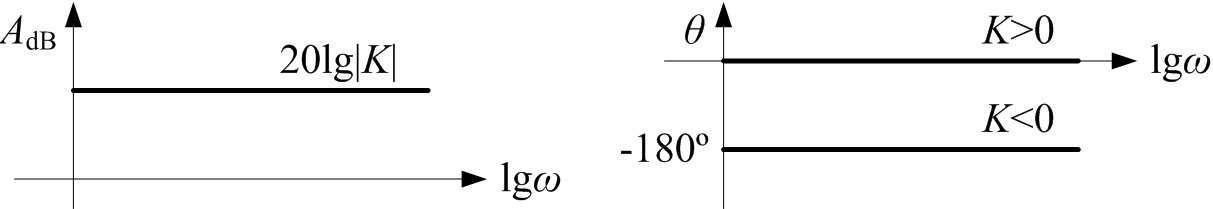
\includegraphics[height=1.8cm]{8.4.2-1.png}
\end{figure}
\[
A_{\mathrm{dB}}=20\lg \left| K \right| \qquad \qquad \theta =\mathrm{arc}\tan \frac{0}{K}=\begin{cases}
	0 &K>0\\
	-\pi &K<0\\
\end{cases}
\]

~

{\bf 因子$i\omega $}

当出现在分子多项式中时,增益为斜率20dB/10倍频的过$\left( 1,0 \right) $的上升直线,相位稳定在$\pi /2$。

\begin{figure}[ht]
\centering
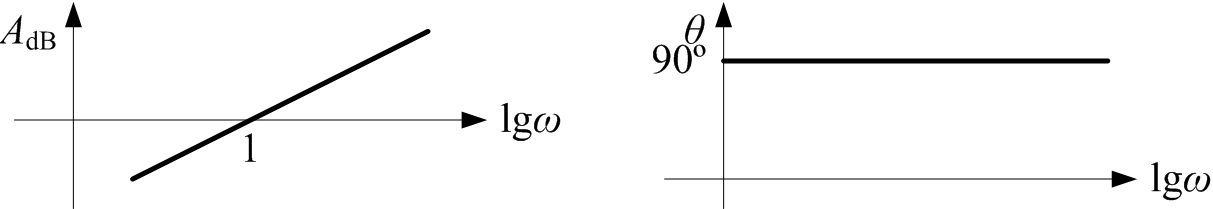
\includegraphics[height=1.8cm]{8.4.2-2.png}
\end{figure}
\[
A_{\mathrm{dB}}=20\lg \left| i\omega \right|=20\lg \omega \qquad \qquad \theta =\mathrm{arc}\tan \frac{\omega}{0}=\frac{\pi}{2}
\]

当出现在分母多项式中时,增益为斜率-20dB/10倍频的过$\left( 1,0 \right) $的下降直线,相位稳定在$-\pi /2$。
\begin{figure}[h]
\centering
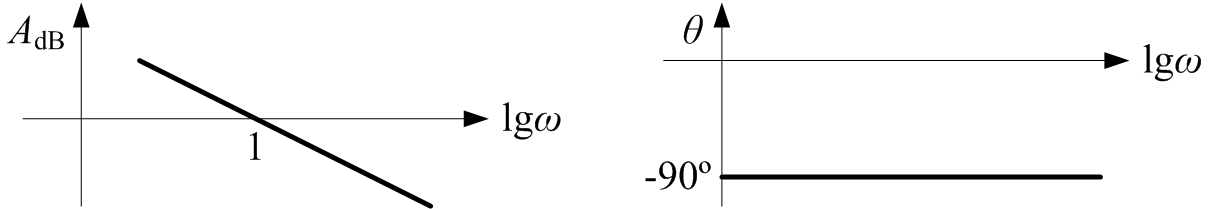
\includegraphics[height=1.8cm]{8.4.2-3.png}
\end{figure}
\[
A_{\mathrm{dB}}=20\lg \left| \frac{1}{i\omega} \right|=-20\lg \omega \qquad \qquad \theta =-\mathrm{arc}\tan \frac{\omega}{0}=-\frac{\pi}{2}
\]

{\bf 因子$i\frac{\omega}{\omega _z}+1$}

当出现在分子多项式中时,增益为0的平行线,过了转角频率 后为斜率为20dB/10倍频的上升直线,相位起初为0,转角频率$\omega _z$处达到$\pi /4$,最后稳定在$\pi /2$。
\begin{figure}[h]
\centering
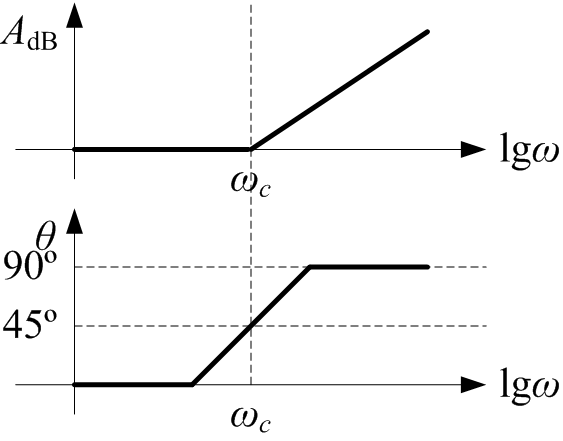
\includegraphics[height=3.5cm]{8.4.2-4.png}
\end{figure}
\begin{align*}
&A_{\mathrm{dB}}=20\lg \left| i\frac{\omega}{\omega _z}+1 \right|=20\lg \sqrt{\left( \frac{\omega}{\omega _z} \right) ^2+1}=\begin{cases}
	0 &\omega <\omega _z\\
	20\lg \frac{\omega}{\omega _z} &\omega >\omega _z\\
\end{cases} \\
&\theta =\mathrm{arc}\tan \frac{\omega}{\omega _z}=\begin{cases}
	0 &\omega <\frac{\omega _z}{10}\\
	\frac{\pi}{4} &\omega =\omega _z\\
	\frac{\pi}{2} &\omega >10\omega _z\\
\end{cases}
\end{align*}

当出现在分子多项式中时,增益为0的平行线,过了转角频率 后为斜率为-20dB/10倍频的下降直线,相位起初为0,转角频率$\omega _z$处达到$-\pi /4$,最后稳定在$-\pi /2$。
\begin{figure}[ht]
\centering
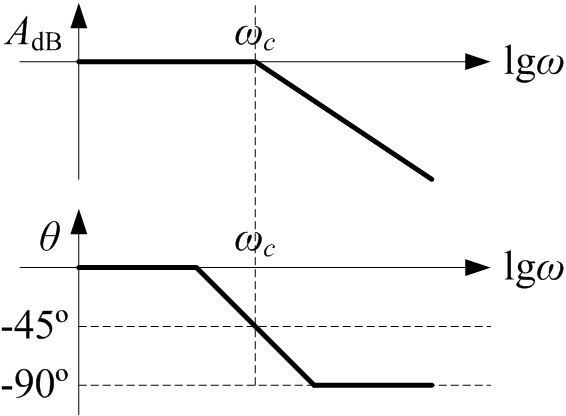
\includegraphics[height=3.5cm]{8.4.2-5.png}
\end{figure}
\begin{align*}
&A_{\mathrm{dB}}=20\lg \frac{1}{\left| i\frac{\omega}{\omega _p}+1 \right|}=-20\lg \sqrt{\left( \frac{\omega}{\omega _p} \right) ^2+1}=\begin{cases}
	0 &\omega <\omega _p\\
	-20\lg \frac{\omega}{\omega _p} &\omega >\omega _p\\
\end{cases} \\
&\theta =-\mathrm{arc}\tan \frac{\omega}{\omega _z}=\begin{cases}
	0 &\omega <\frac{\omega _p}{10}\\
	-\frac{\pi}{4} &\omega =\omega _p\\
	-\frac{\pi}{2} &\omega >10\omega _p\\
\end{cases}
\end{align*}

%============================================================
\subsection{Python应用——scipy.signal.bode函数}

scipy.signal.bode()函数用于生成系统的波特图。
\begin{figure}[h]
\centering
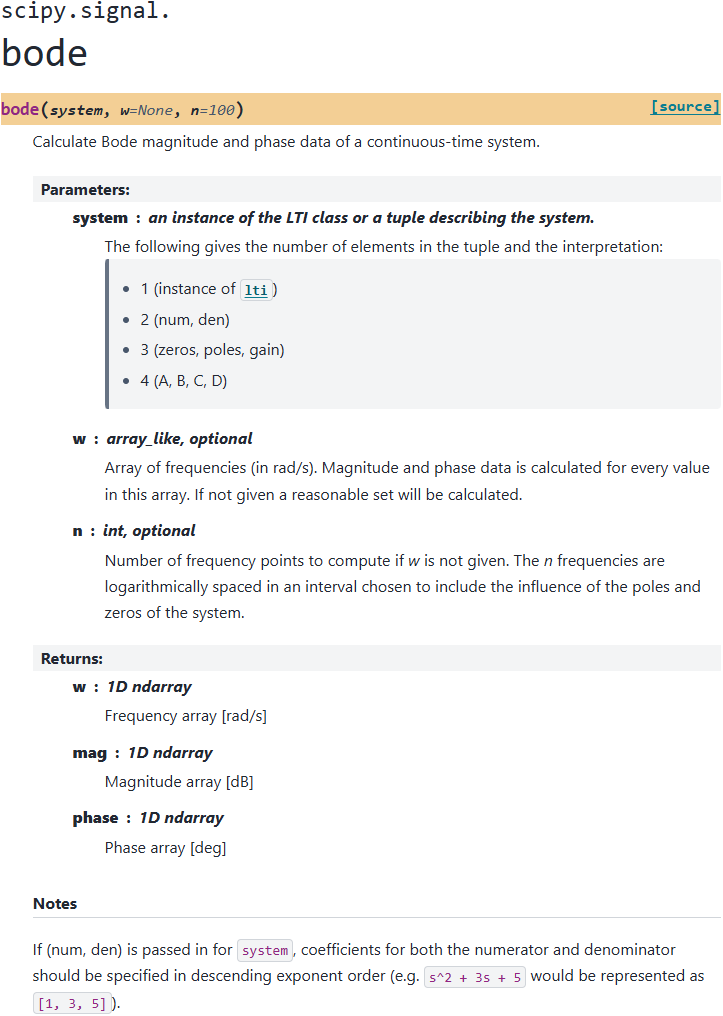
\includegraphics[width=7.5cm]{8.4.3-1.png}
\end{figure}

~

\begin{example}
若系统传递函数$H\left( s \right) =\frac{2}{s+2}$,画波特图。
\end{example}

\begin{python}
H = signal.TransferFunction([2], [1,2])
w = np.arange(0.1, 100, 0.01)
w, mag, phase = H.bode(w=w)

axs[0][0].plot(w, mag);   axs[0][0].set_xscale('log')
axs[1][0].plot(w, phase); axs[1][0].set_xscale('log')
axs[0][1].plot(w, mag)
axs[1][1].plot(w, phase)
\end{python}

\begin{figure}[h]
\centering
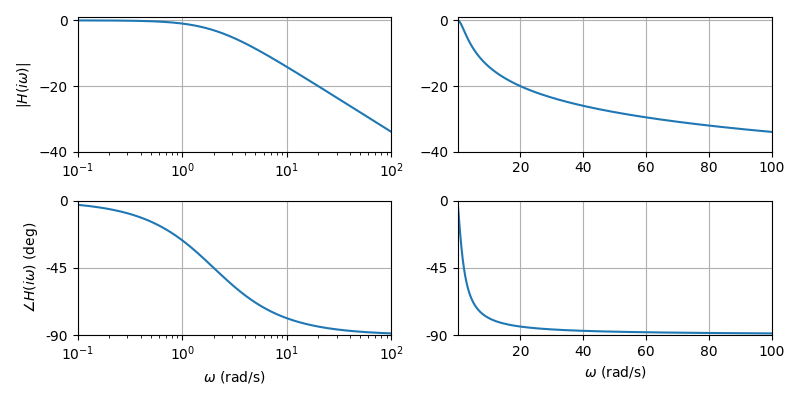
\includegraphics[height=5cm]{8.4.3-2.png}
\end{figure}






\newpage
\section{本章小结}

本章着重介绍传递函数的应用:稳定性判断和频率响应函数。

在设计系统时,首先可以通过稳定性判断获得一个系统的初步构架,即初步设计一个稳定的n阶系统。
然后通过频率响应函数进一步调整系统,达到对信号的处理。
由于信号可以看成无数频率分量的叠加(FT),而系统又可以通过频率响应函数描述,所以很容易使用频率响应函数调整系统的带宽、中频增益、延迟等一系列指标。
系统的各项指标在频率响应函数下的物理意义十分清晰,而且处理上,也是简单的算术运算。
这就是LT在工程上的意义。









